\documentclass{beamer}
\usepackage[frenchb]{babel}
\usepackage[utf8]{inputenc}
\usepackage[T1]{fontenc}
\usepackage{babel}
\usepackage{graphicx}
\usepackage{amsmath}
\usepackage{caption}
\usepackage{subcaption}
\usepackage{siunitx}
\usepackage{textcomp}
\usepackage{xcolor}
\usepackage[T1]{fontenc}
\usepackage[utf8]{inputenc}
\usepackage{tikz}
\usetikzlibrary{quotes,angles,calc,intersections,babel,through,backgrounds,angles,positioning}
\usepackage{rotating}

\usetheme{Warsaw}

\title{Goutte soufflée : croissance et dynamique d'une goutte cisaillée par un écoulement d'air\xspace}
\author{BESSENG A IREH Guy Raymond}
\institute[]{Université Paul Sabatier}
\date{21 Mars 2018}
\setbeamertemplate{caption}{\raggedright\insertcaption\par}
\addtobeamertemplate{navigation symbols}{}{%
    \usebeamerfont{footline}%
    \usebeamercolor[fg]{footline}%
    \hspace{1em}%
    \insertframenumber/\inserttotalframenumber
}
\begin{document}

\maketitle
%************************************************
\section{Introduction}\label{sec:introduction}
%************************************************
\begin{frame}
\frametitle{Introduction}
\begin{center}
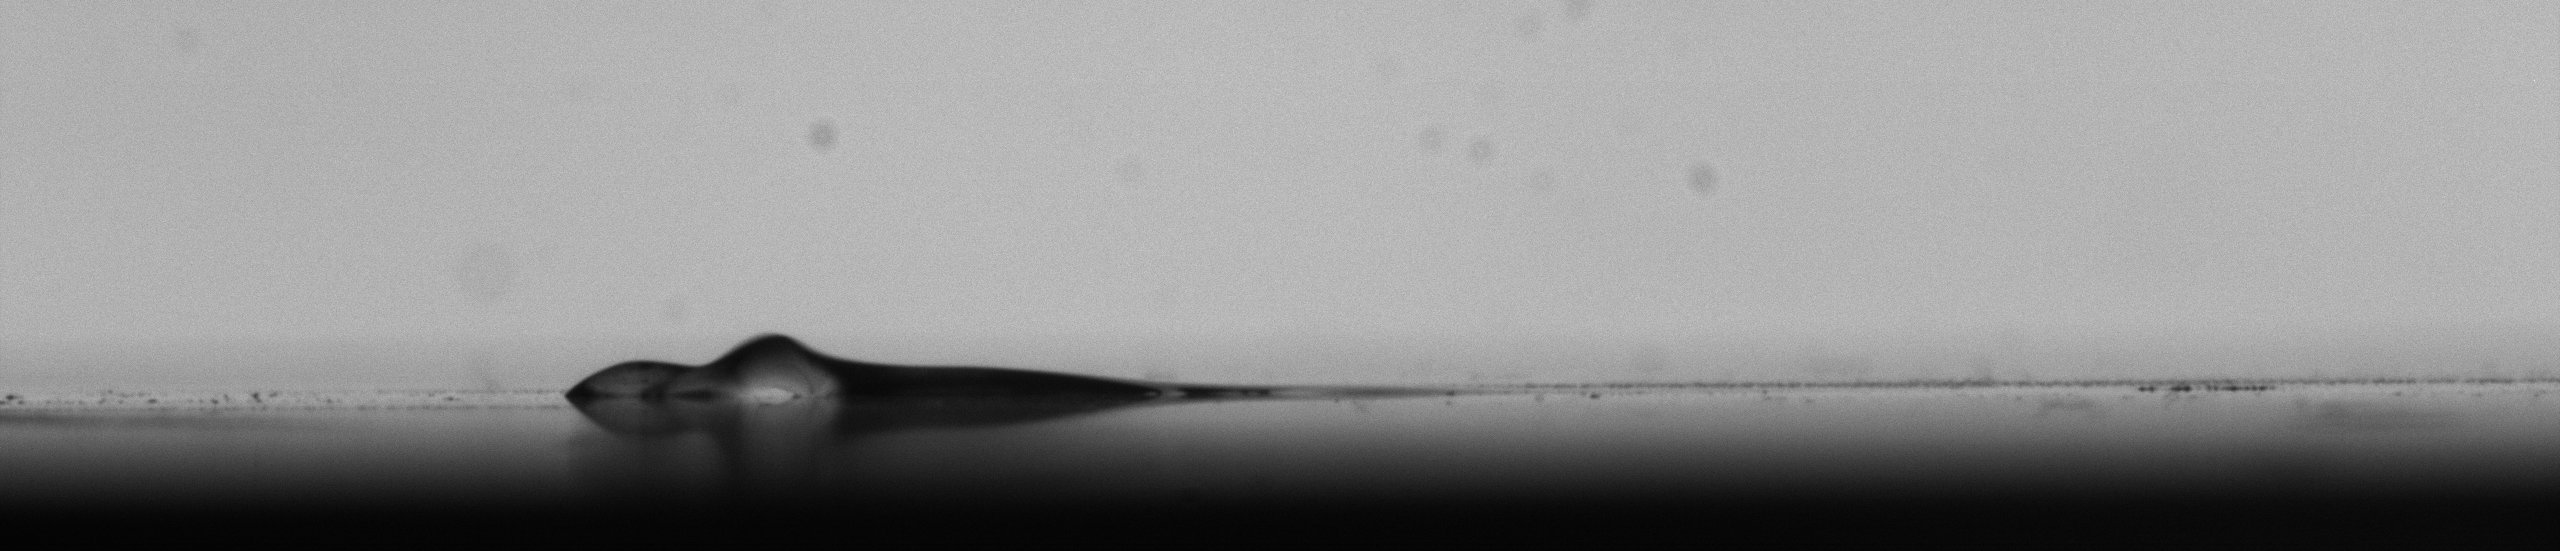
\includegraphics[height=0.2\linewidth]{./image/test628.jpg} \\ 
\end{center}
\end{frame}


%************************************************
\section{Couche limite}\label{sec:couche}
%************************************************
\begin{frame}
\frametitle{Hypothèses}
\begin{itemize}
\item Écoulement bidimensionnel, stationnaire
\item $u \sim U$, $v \sim V$, $x \sim L$, $y \sim \delta$
\item $\frac{\delta}{L} << 1$
\end{itemize}
\begin{align}	
	\frac{\partial u}{\partial x} 
	+
	\frac{\partial v}{\partial y} 
	&= 0 \\
	u\frac{\partial u}{\partial x} + 
	v\frac{\partial u}{\partial y} 
	&= - \frac{1}{\rho}
	\frac{\partial p}{\partial  x} +
	\nu
	\frac{\partial^{2} u}{\partial  y^{2}} \\
	\frac{\partial p}{\partial y} 
	&= 0
\end{align}
\end{frame}

%************************************************
\subsection{Couche limite de Blasius}\label{sub:Blasius}
%************************************************
\begin{frame}
\frametitle{Couche limite de Blasius}
\begin{itemize}
\item Écoulement bidimensionnel, stationnaire
\item $u \sim U$, $v \sim V$, $x \sim L$, $y \sim \delta$
\item $\frac{\delta}{L} << 1$
\end{itemize}
\begin{align}	
	\frac{\partial u}{\partial x} 
	+
	\frac{\partial v}{\partial y} 
	&= 0 \\
	u\frac{\partial u}{\partial x} + 
	v\frac{\partial u}{\partial y} 
	&= - \frac{1}{\rho}
	\frac{\partial p}{\partial  x} +
	\nu
	\frac{\partial^{2} u}{\partial  y^{2}} \\
	\frac{\partial p}{\partial y} 
	&= 0
\end{align}
\end{frame}

%************************************************
\subsection{Comparaisons Blasius et expérience}\label{sec:comparaison}
%************************************************
\begin{frame}
\frametitle{Couche limite de Blasius}
\begin{center}
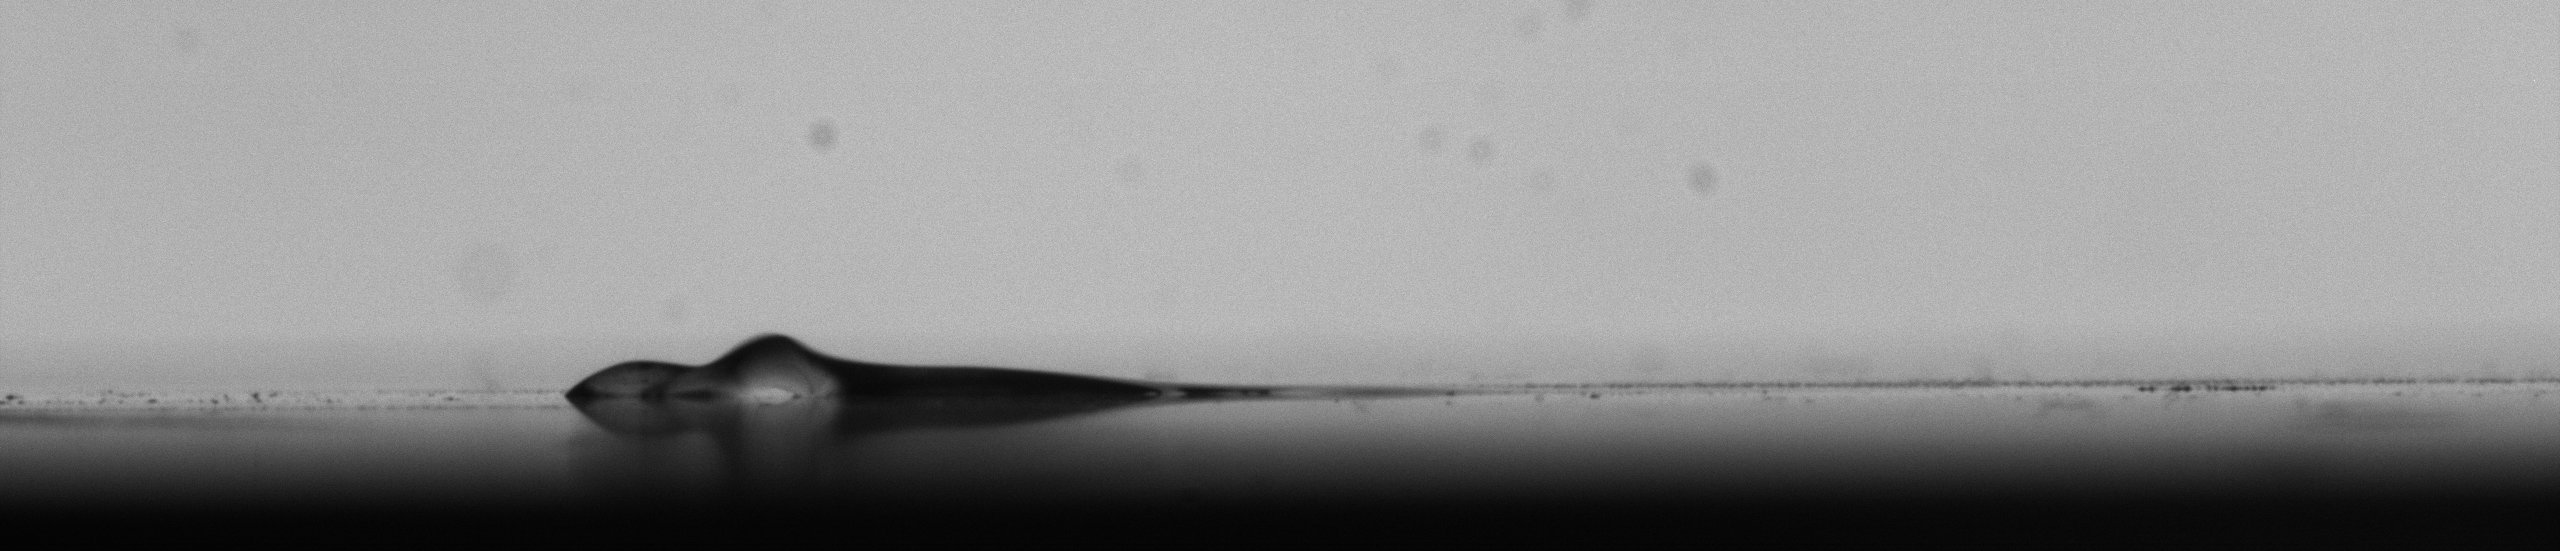
\includegraphics[height=0.2\linewidth]{./image/test628.jpg} \\ 
\end{center}
\end{frame}


%************************************************
\section{Capillarité}\label{sec:couche}
%************************************************


%************************************************
\section{Expériences}\label{sec:experience}
%************************************************
\begin{frame}
\frametitle{Résutats}
\begin{figure}[!ht]
	\centering
		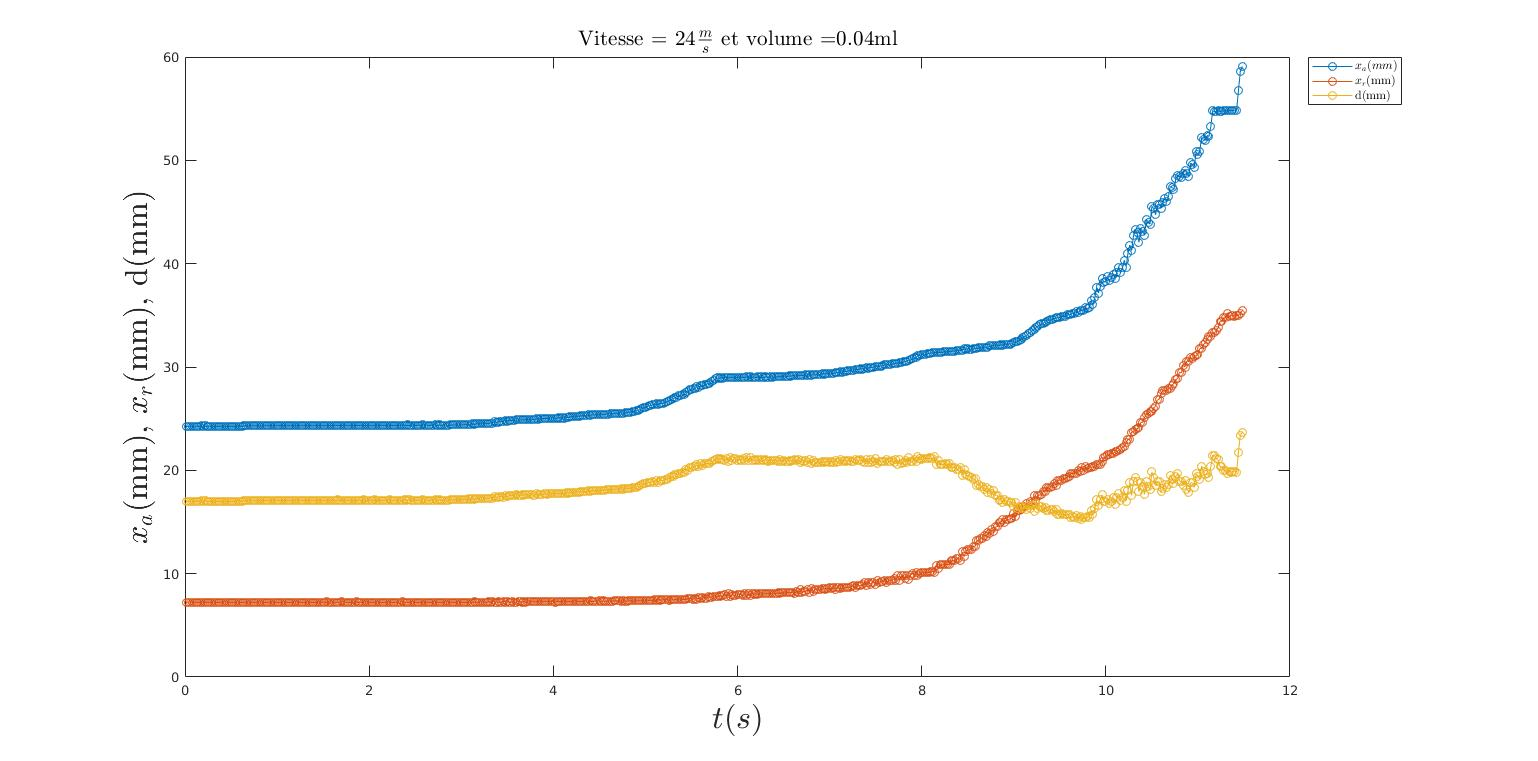
\includegraphics[width=\linewidth]{./image/v=24_vol=004_xaxrd.jpg}
		\caption{$\textcolor{blue}{x_{a}}$,
		$\textcolor{red}{x_{r}}$, $\textcolor{yellow}{d}$, 
		$U_{\infty}=24m.s^{-1}$, \\
                volume =$0.04ml$}
		\label{fig:entre_xaxrd}
		 \end{figure}
\end{frame}
\begin{frame}
\frametitle{Résutats}
\begin{figure}[!ht]
		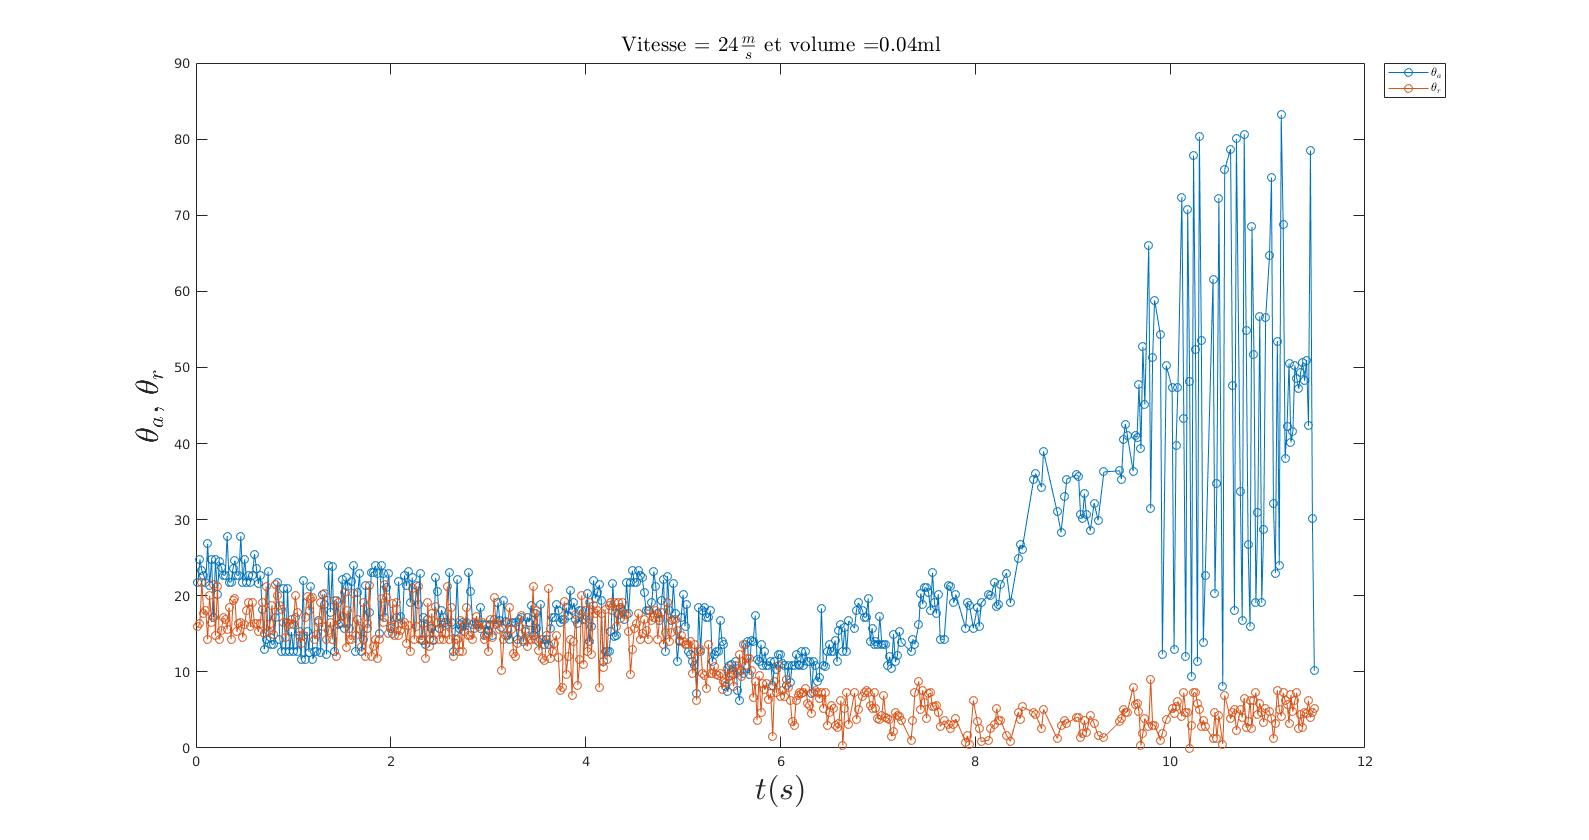
\includegraphics[width=\linewidth]{./image/v=24_vol=004_oaor.jpg}
		\caption{$\textcolor{blue}{\theta_{a}}$,
		$\textcolor{red}{\theta_{r}}$, $U_{\infty}=24m.s^{-1}$, volume =$0.04ml$}
		\label{fig:entre_oaor}
 \end{figure}
\end{frame}
\begin{frame}
\frametitle{Résutats}
\begin{figure}[!ht]
		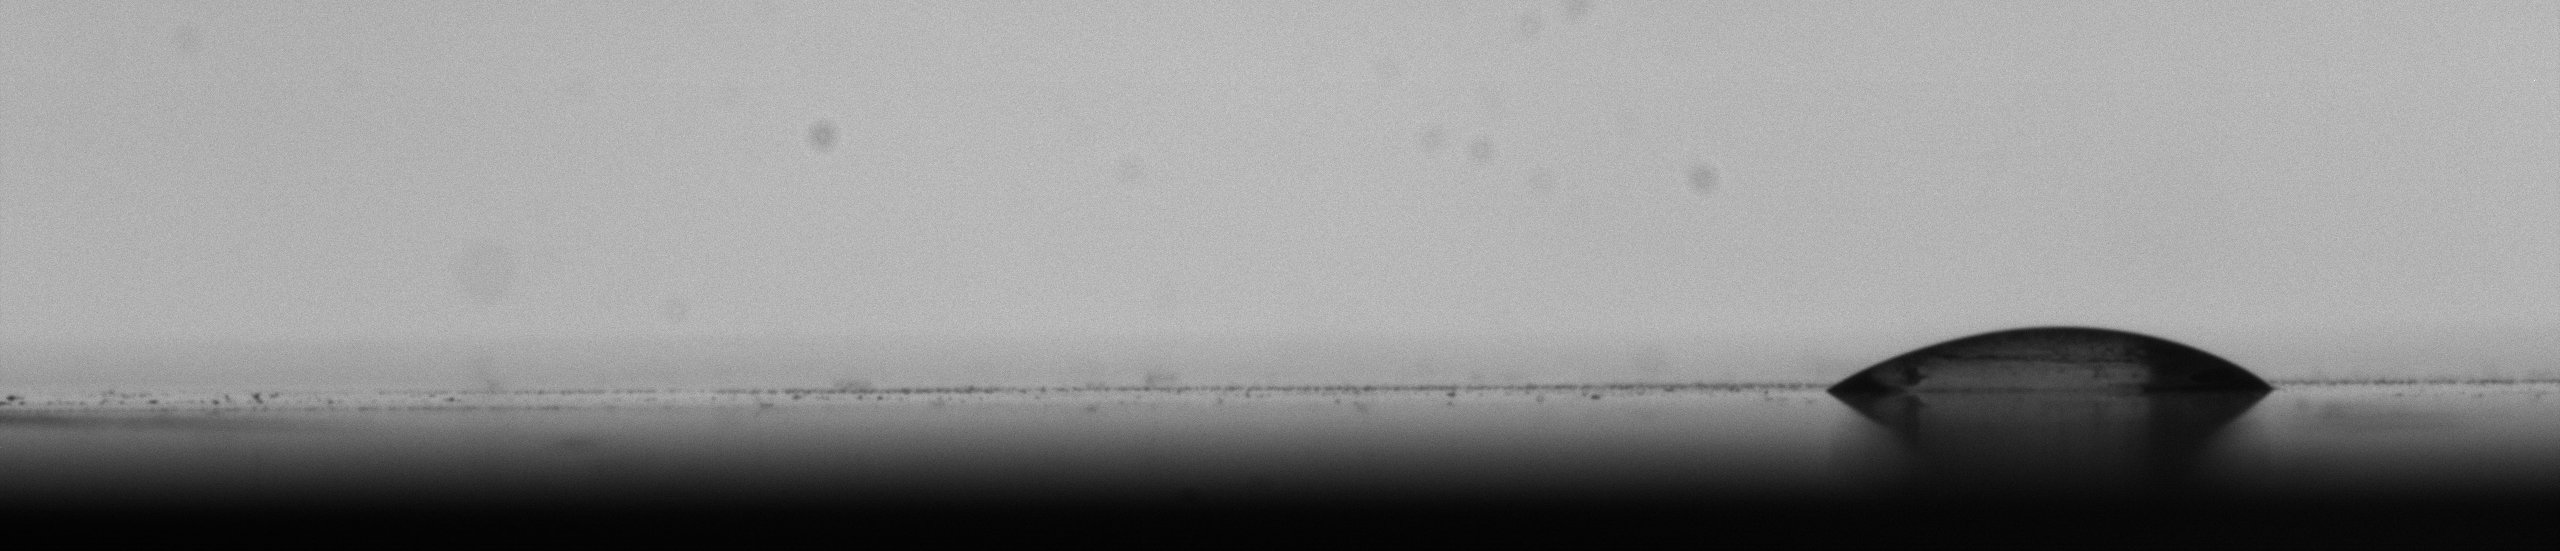
\includegraphics[width = 0.35\linewidth]{./image/test.jpg}\\
		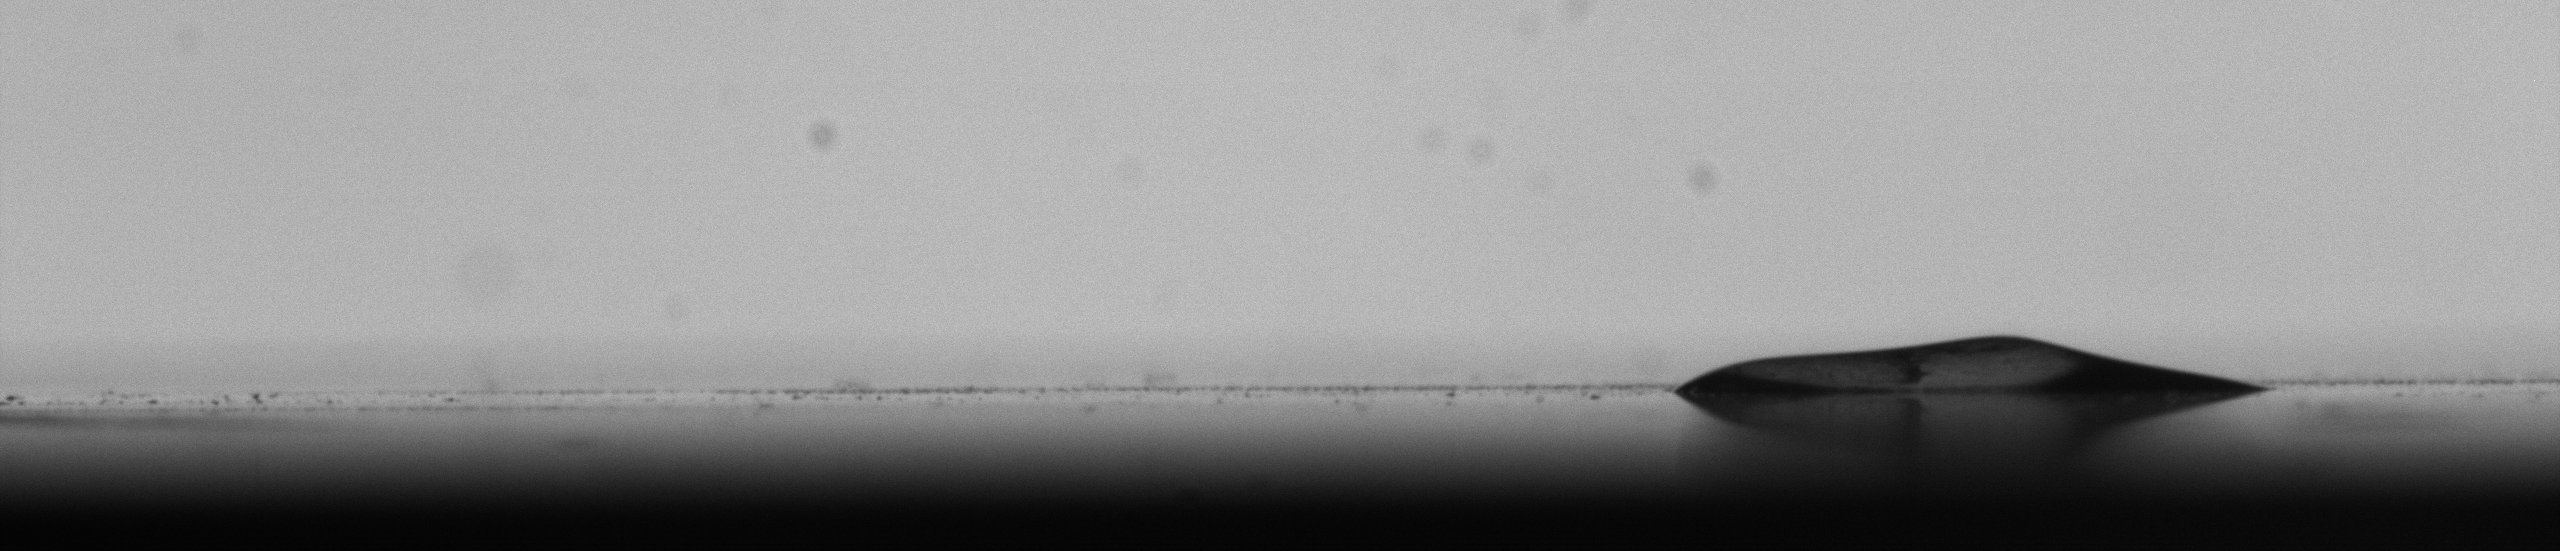
\includegraphics[width = 0.35\linewidth]{./image/test400.jpg}\\
		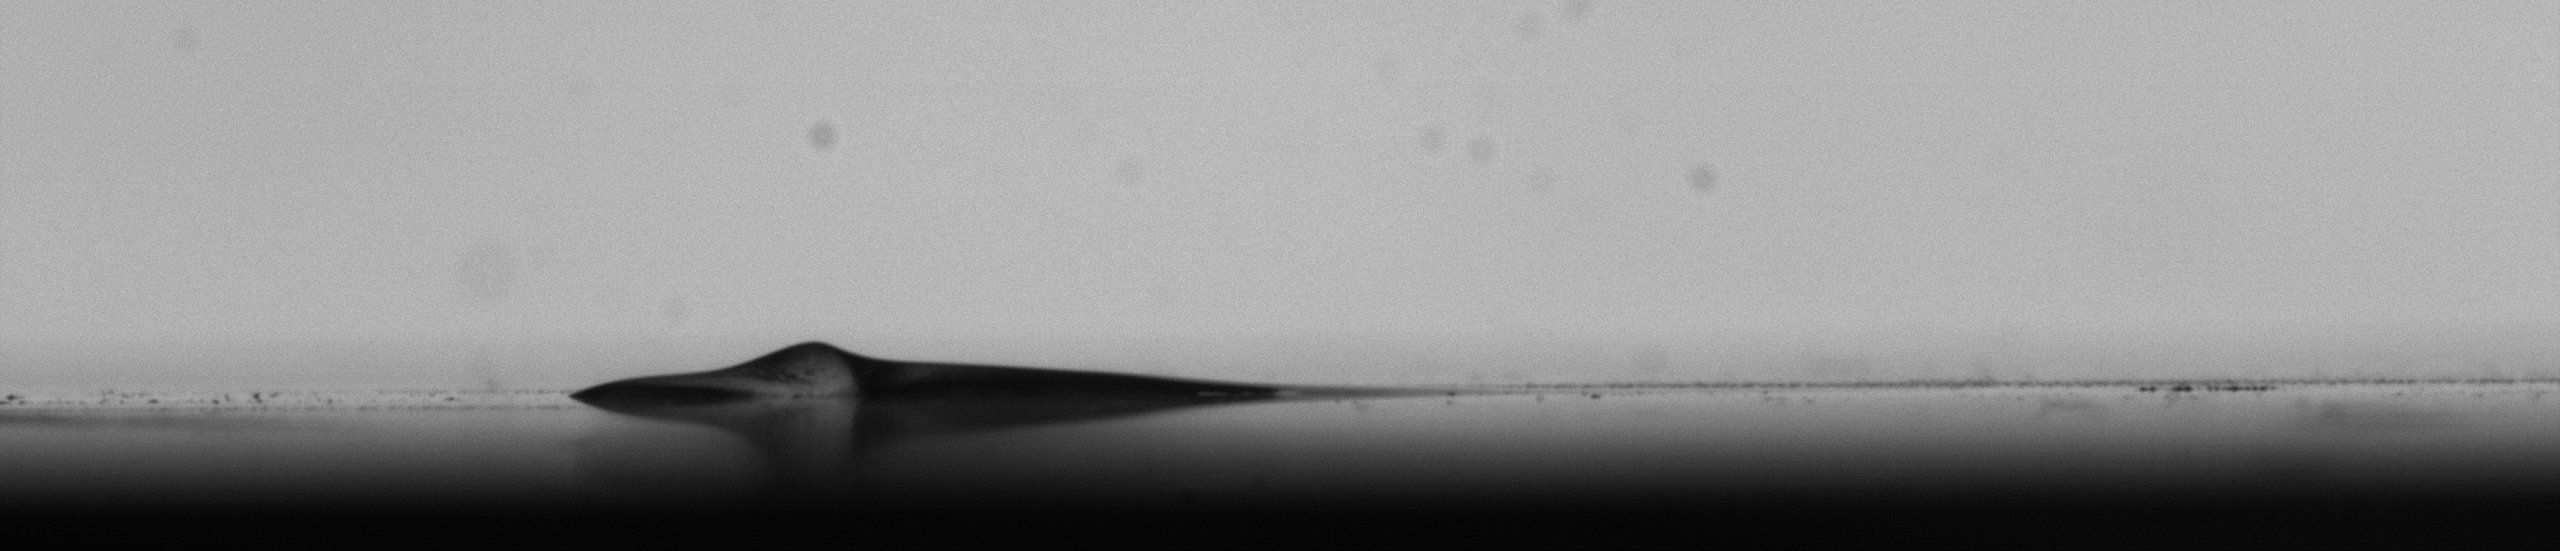
\includegraphics[width = 0.35\linewidth]{./image/test626.jpg}\\
		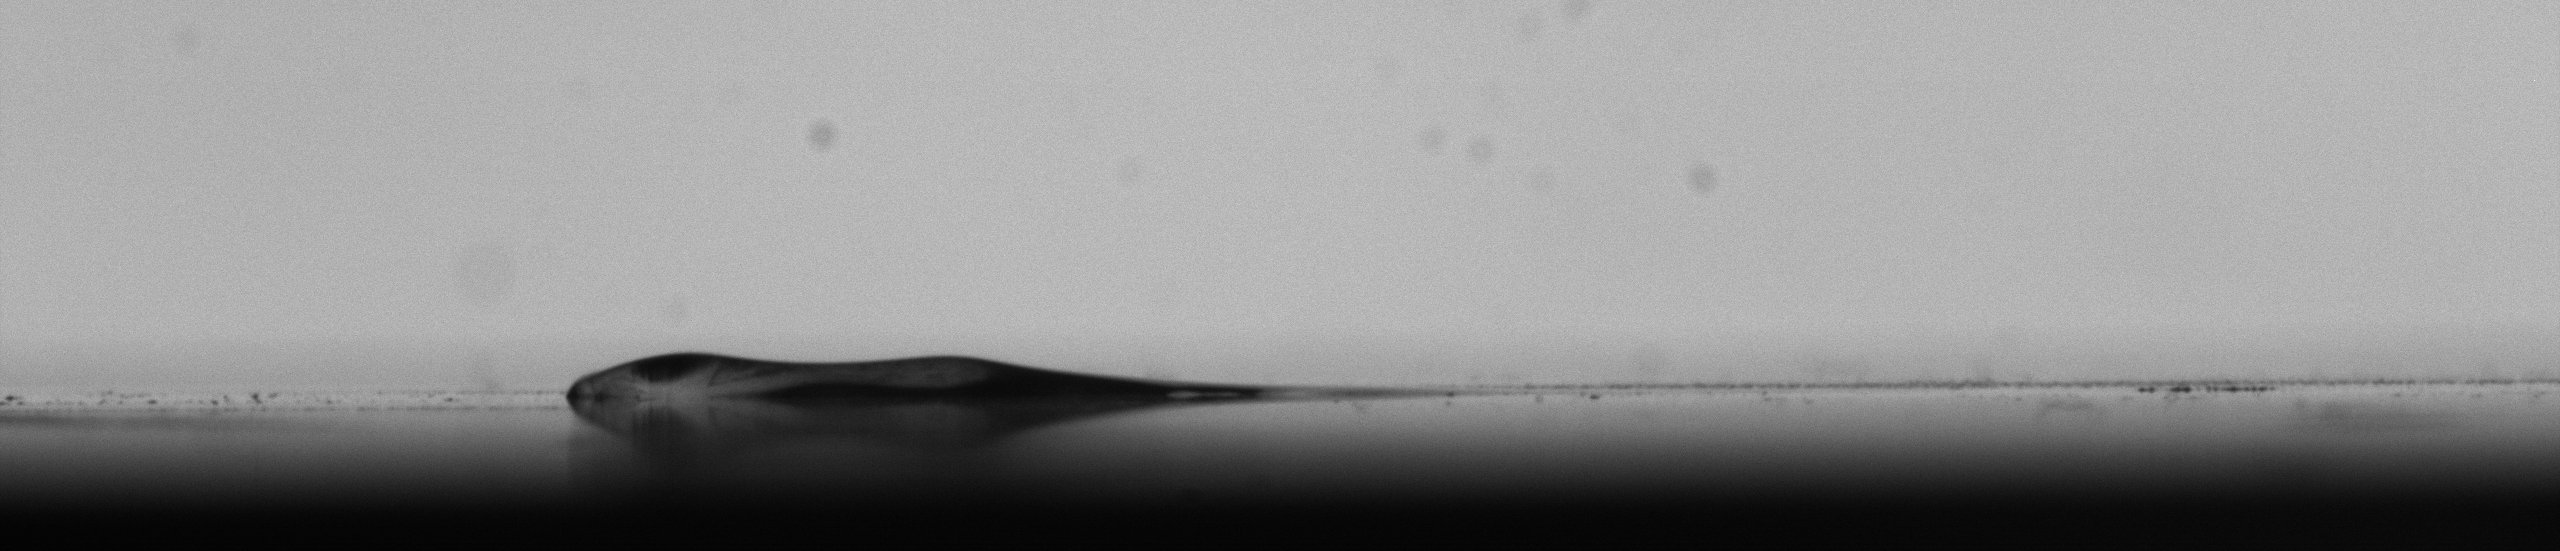
\includegraphics[width = 0.35\linewidth]{./image/test627.jpg}\\
		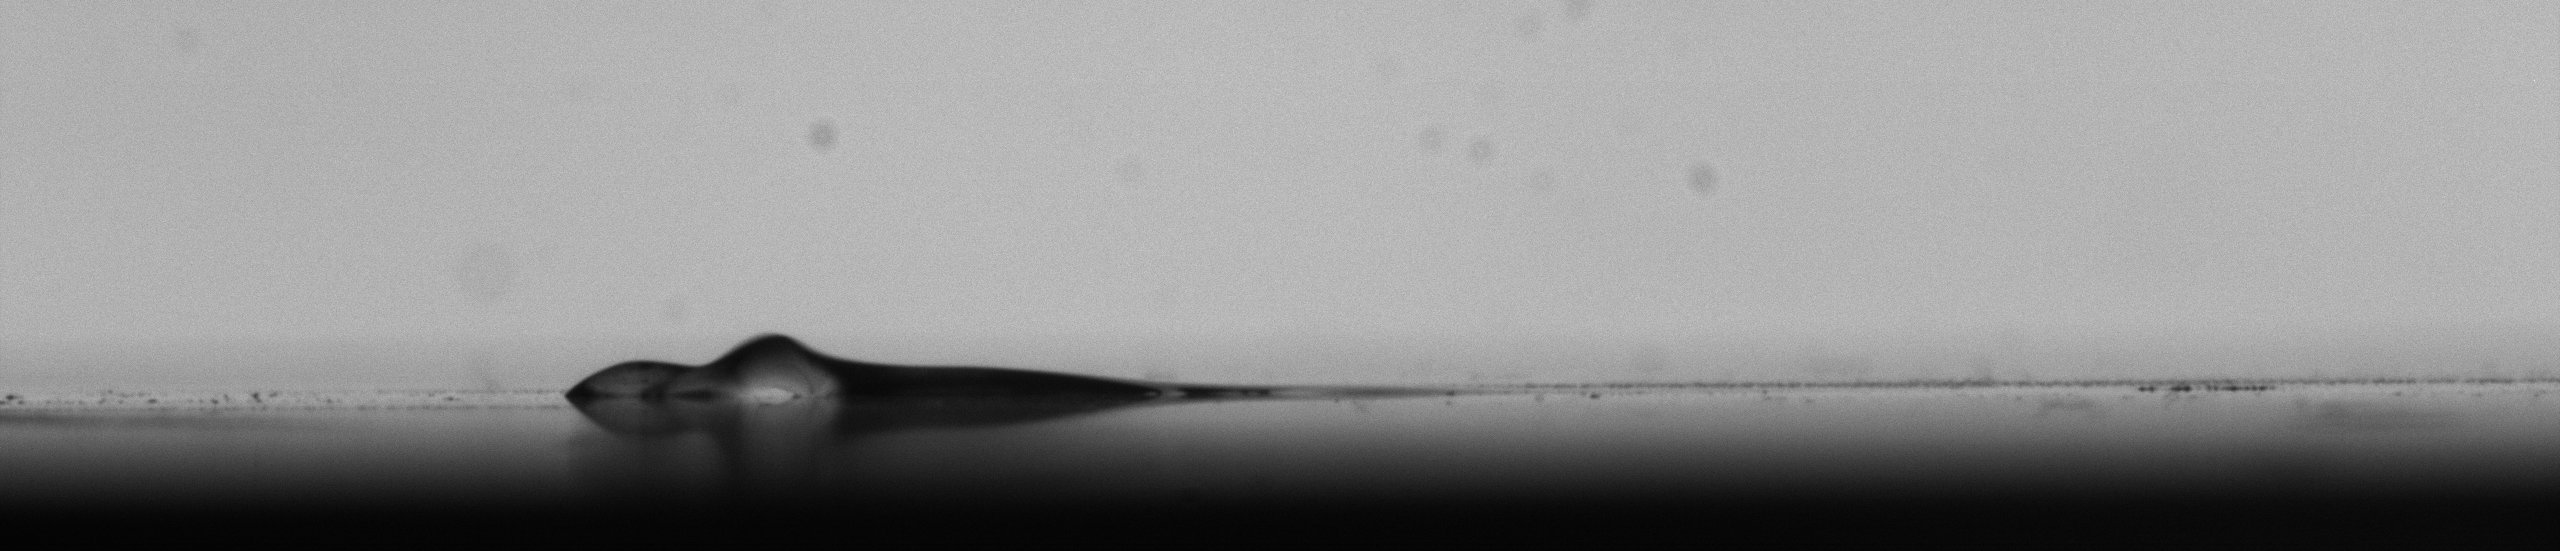
\includegraphics[width = 0.35\linewidth]{./image/test628.jpg}\\
		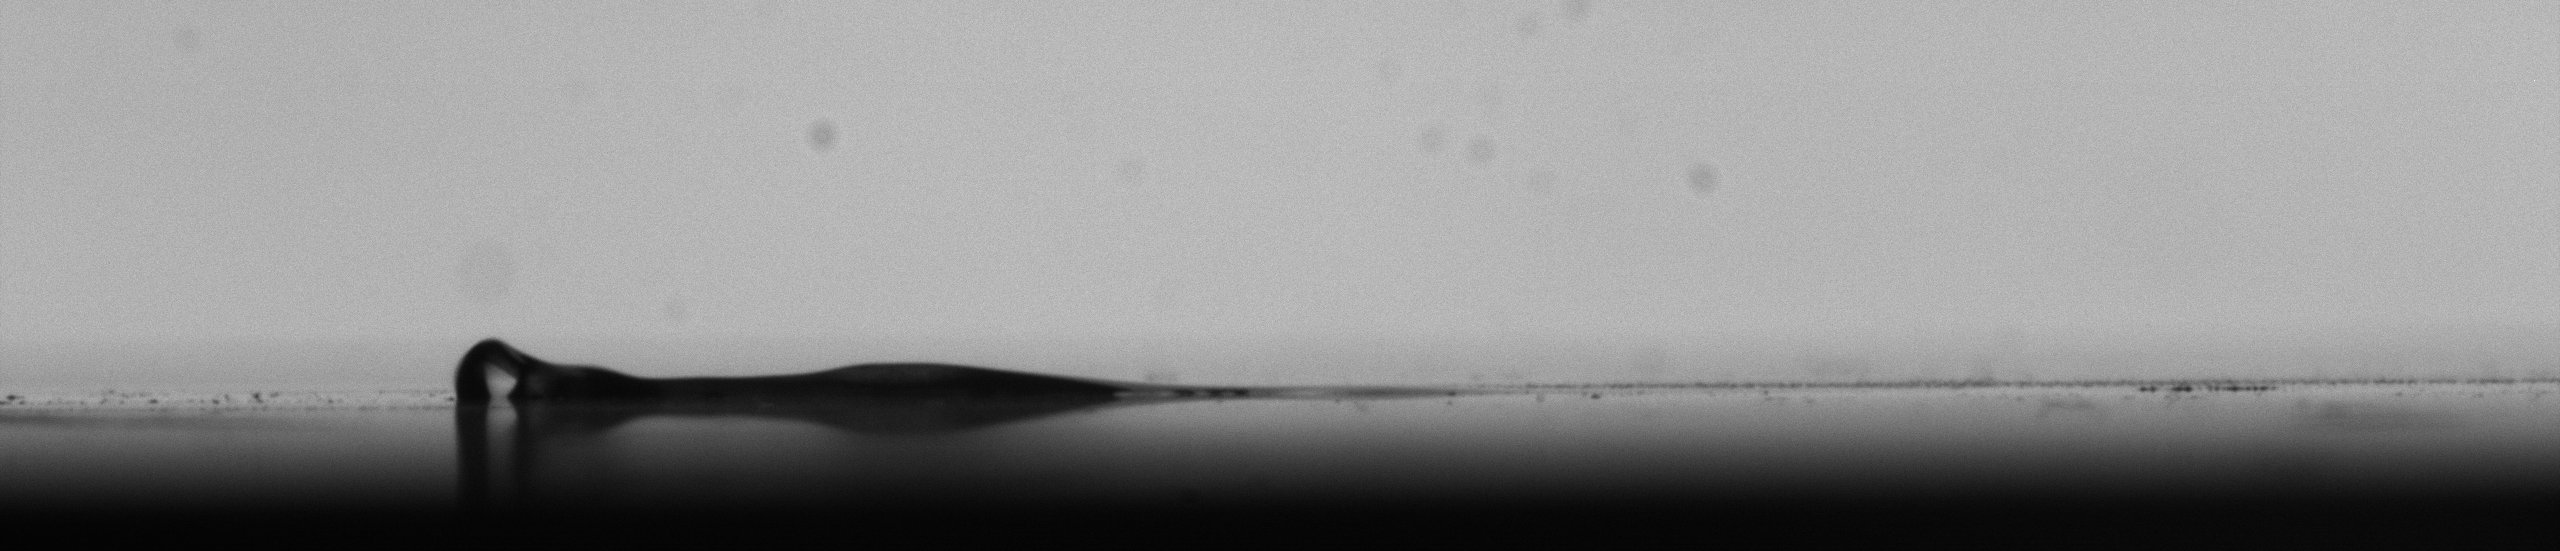
\includegraphics[width = 0.35\linewidth]{./image/test629.jpg}
	\caption{$U_{\infty}=20m.s^{-1}$, de haut en bas nous avons :\\
	$t = ~0s,~8s,~12.52s,~12.54s,~12.58s$}
		\label{fig:test}
\end{figure}
\end{frame}

\begin{frame}
\frametitle{Résutats}
\begin{figure}[!ht]
        \centering
		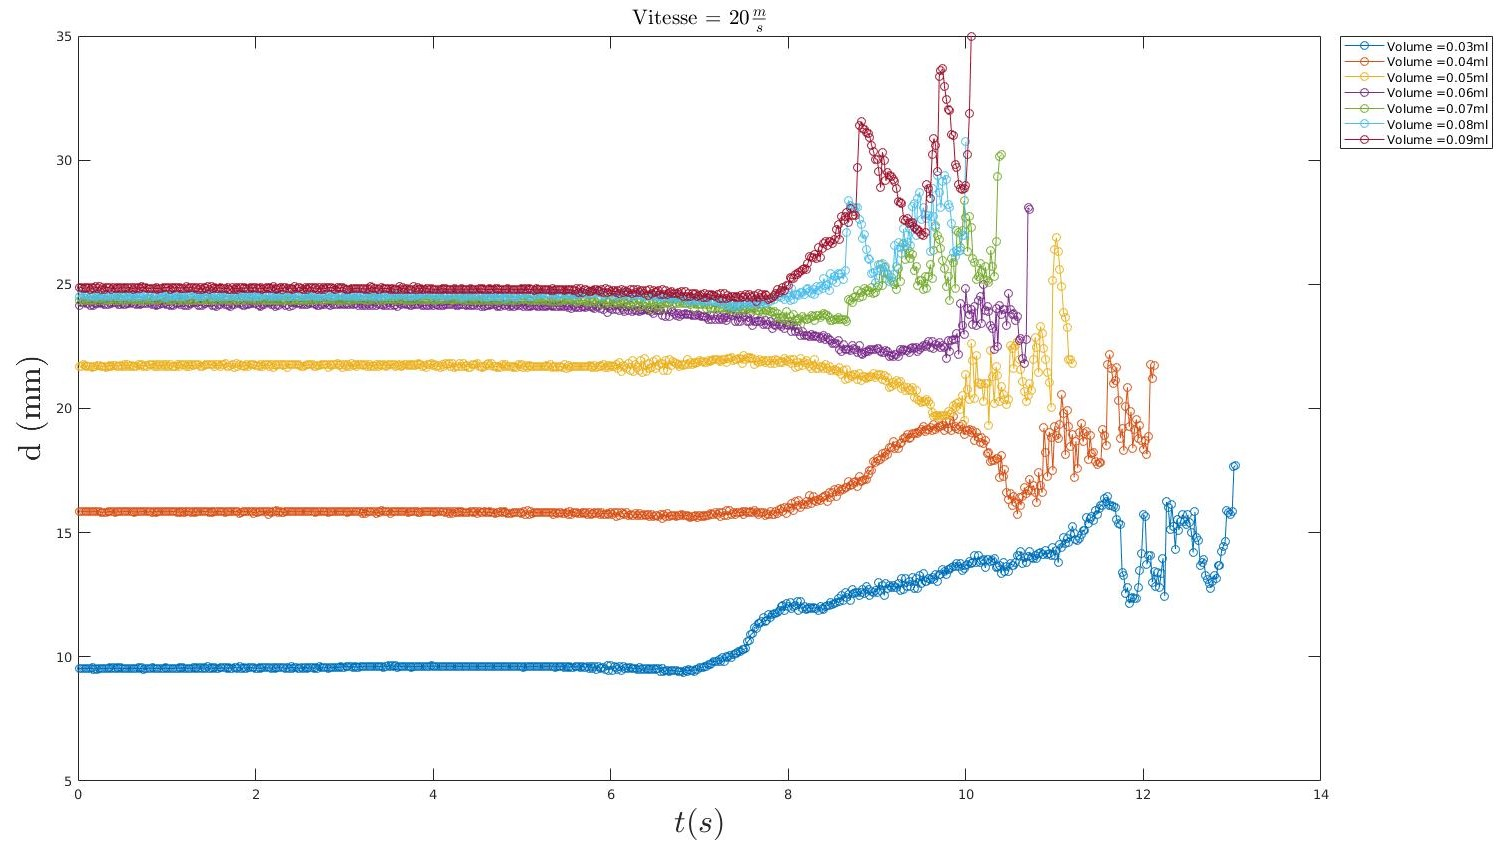
\includegraphics[width = \linewidth]{./image/v=20d.jpg}
	\caption{$d$, $U_{\infty}=20m.s^{-1}$}
		\label{fig:v=20d}
\end{figure}
\end{frame}

\begin{frame}
\frametitle{Résutats}
\begin{figure}[!ht]

	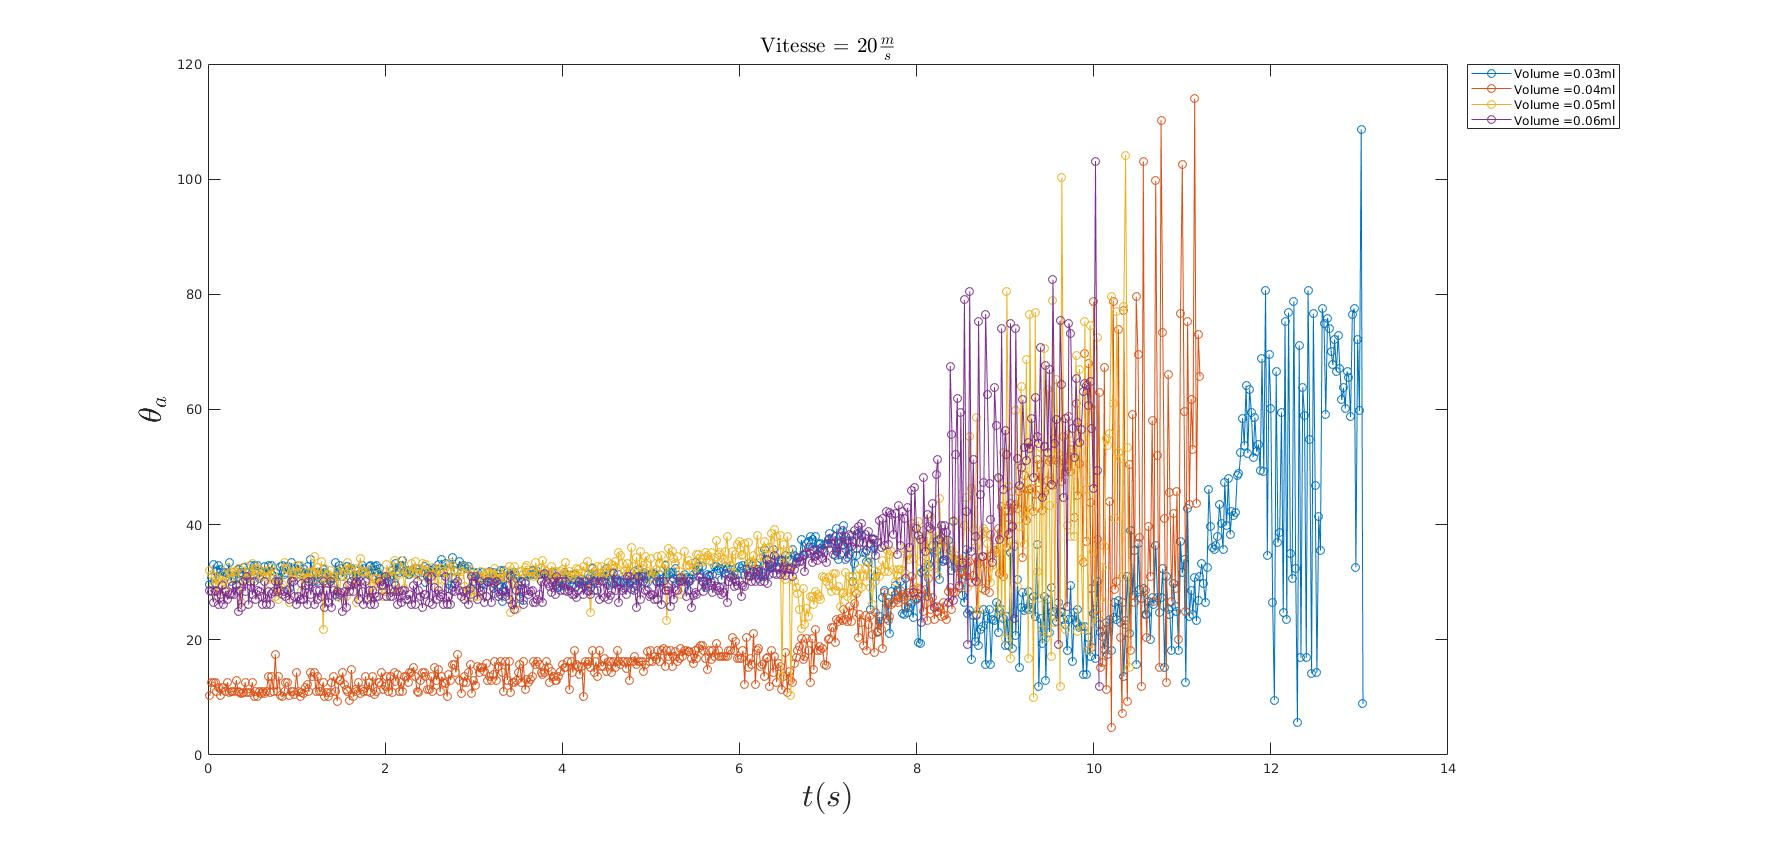
\includegraphics[width = \linewidth]{./image/v=20oa_2.jpg}
	\caption{$\theta_{a}$, $U_{\infty}=20m.s^{-1}$}
		\label{fig:v=20oa_2}
\end{figure}
\end{frame}

\begin{frame}
\frametitle{Résutats}
\begin{figure}[!ht]
        \centering
	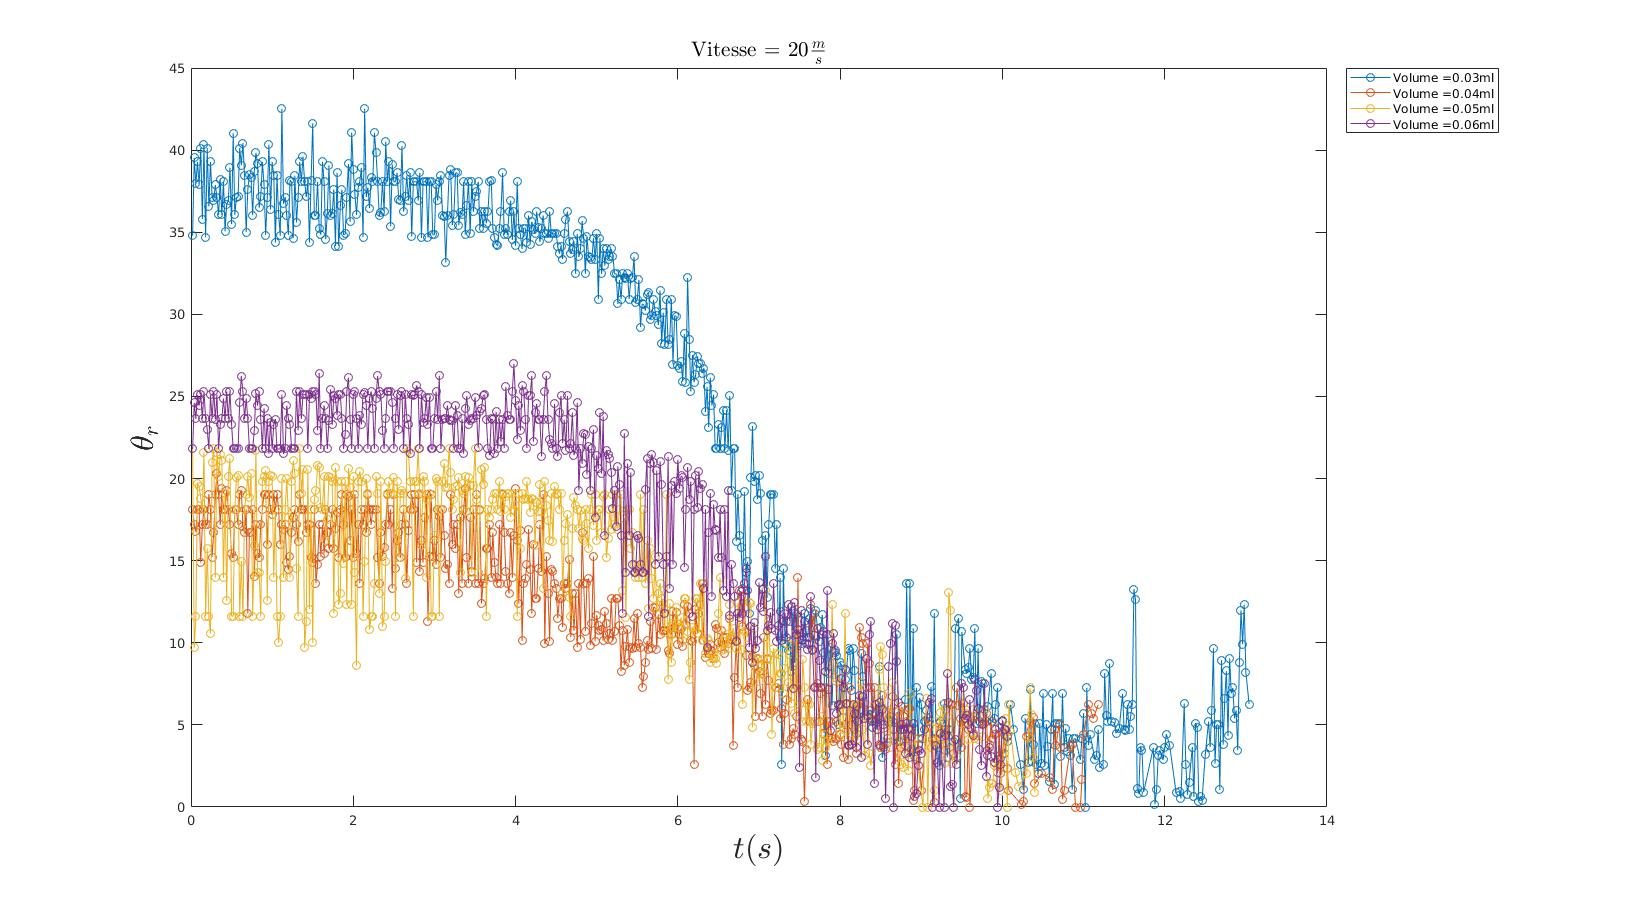
\includegraphics[width = \linewidth]{./image/v=20or_2.jpg}
	\caption{$\theta_{r}$, $U_{\infty}=20m.s^{-1}$}
		\label{fig:v=20or_2}
\end{figure}
\end{frame}

\begin{frame}
\frametitle{Questions}
  \center{Avez-vous des questions ?}
\end{frame}



\end{document}
